% Panorama

% Un cuarto propio conectado. Remedios Zafra > Pdf revisar para referencias 

\documentclass[11pt,letterpaper]{article}
\usepackage[utf8]{inputenc}
\usepackage[spanish]{babel}
\usepackage{endnotes}
\usepackage{xurl}
%\usepackage[hyphens]{url}
\usepackage{hyperref}
\usepackage{amsmath}
\usepackage{amsfonts}
\usepackage{amssymb}
%\usepackage[final]{changes}
\usepackage{graphicx}
\usepackage{float}
\usepackage[dvipsnames]{xcolor}
\usepackage{changes}
\usepackage[sort&compress]{natbib}
\usepackage{marginnote}
% \usepackage{xcolor}
\usepackage{subfig}
% \usepackage[top=Bcm, bottom=Hcm, outer=Ccm, inner=Acm, heightrounded, marginparwidth=Ecm, marginparsep=Dcm]{geometry}
\usepackage{changes}
%% Use "final" option to remove all tracking markups
% \usepackage[final]{changes}

\definechangesauthor[color=Red]{MT}
\definechangesauthor[color=Green]{EO}
\definechangesauthor[color=Blue]{DS}

\renewcommand{\notesname}{Notas}

\hypersetup{
    colorlinks=true,
    linkcolor=magenta,
    filecolor=magenta,      
    urlcolor=magenta,
    citecolor=magenta,
}

\urlstyle{same}

\author{Marianne Teixido, Dorian Sotomayor, Emilio Ocelotl}
%\title{Panorama. Tecnologías libres e inmersivas para el performance audiovisual}

\title{%
  Panorama \\
  \large Escritura de espacios libres e inmersivos para el performance audiovisual}

% Las siguientes líneas habilitan las palabras clave

\providecommand{\keywords}[1]
{
  \small	
  \textbf{\textit{Palabras clave---}} #1
}

\let\footnote=\endnote

\begin{document}

\maketitle

%\begin{abstract}
%  
El confinamiento provocado por la pandemia de COVID-19 obligó a artistas, gestores, instituciones públicas e industrias a replantear maneras de compartir flujos co-presenciales y hacer performance audiovisual en vivo. La presente investigación se enmarca en está búsqueda; el distanciamiento social forzado fue el pretexto para resolver necesidades tecnológicas que pudieran equilibrar la perspectiva funcional y la experimental. Este trayecto desembocó en discusiones sobre materialidad y virtualidad.                          

El presente artículo describe \textit{Panorama}\footnote{Repositorio de Panorama.}, un conjunto de módulos de código y software que permiten realizar conciertos en espacios virtuales, tridimensionales alojados en la web. La hipótesis/premisa central de este proyecto buscó que los usuarios pudieran compartir una experiencia ligera para el navegador de manera co-presencial, aprovechando las posibilidades de las tecnologías de transmisión de audio y video.  

%\end{abstract}

%
\keywords{Transmisión, streaming, multiplayer, 3d, espacio, audio, video, materialidad, virtualidad, cyborg}


% Pensar en sustituir el resumen con una introducción 

\section*{Resumen}

El confinamiento provocado por la pandemia de COVID-19 \added[id=EO,comment={Cambié obligó por permitió}]{permitió} a artistas, gestores, instituciones públicas e industrias a replantear maneras de compartir flujos co-presenciales y hacer performance audiovisual en vivo. % Cambié obligó por permitió 

El presente artículo describe \textit{Panorama}, un conjunto de módulos de código y software que permiten realizar conciertos en espacios virtuales tridimensionales alojados en la web.

De manera complementaria, introduce discusiones que surgieron durante la activación del espacio sobre materialidad, virtualidad, descentralización, distribución, arqueologías del ciberespacio, entre otros.                       


\section*{Ecosistema}

\textit{Panorama} \citep{panorama} fue un programa escrito por \textit{PiranhaLab}\footnote{``PiranhaLab es un laboratorio interdisciplinario que trabaja en las tripas del software''. \url{https://piranhalab.github.io/} (Consultado el \today)}, implementado en el marco de conciertos realizados en la web. La premisa central de este proyecto fue escribir una serie de módulos de software para que los asistentes a eventos performáticos audiovisuales pudieran compartir una experiencia ligera para el navegador de manera co-presencial, aprovechando las posibilidades de las tecnologías de transmisión de audio y video. % Primero la hipotesis de trabajo  

La presente investigación hace referencia a casos del ciclo de conciertos \textit{EDGES}, plataforma de experimentación y difusión de proyectos audiovisuales en vivo, impulsada por el Laboratorio de Imágenes en Movimiento del Centro Multimedia del Centro Nacional de las Artes.\footnote{\url{https://www.facebook.com/events/209679013466792} (Consultado el \today)}. Los conciertos realizados en este ciclo se llevaron a cabo del 6 de agosto al 19 de noviembre de 2020.

% Algunos eventos independientes que fueron significativos para la escritura sucedieron poco antes o después de estas fechas.

% Comenté lo siguiente, esto antes era parte de un resumen extenso, ahora parece redundante

% El artículo aporta elementos a una discusión para la reflexión transversal (técnica, estética y  de investigación académica) y utiliza conceptos que nos permiten desplazarnos entre estos hilos para entretejer la investigación transdisciplinaria. Se adscribe a los planteamientos de los estudios del software y busca extender la discusión del terreno técnico y descriptivo. A lo largo del texto buscamos problematizar el papel que juega la computadora (local o en servidores) en la realización de prácticas performáticas y audiovisuales en la web.

%% La discusión inicia con la idea del software como una prótesis y termina problematizando las ideas que orbitan en torno a la cajanegrización de cara a la idea del trabajo socialmente invertido para la escritura de software. % Esto puede ir en discusión 

% Pendiente: cómo resolvemos el problema de ser gestores, artistas y escritores. Investigación artística

% Segundo pendiente: realmente tenemos la capacidad narrativa de plantear una navegación 

% \subsection*{Ecosistema} % Esto antes se llamaba antecedentes ivaciones paralelasun titulo más serio sería: activaciones paralelas

\textit{Panorama} se insertó en un ecosistema que tuvo en común el diseño de la presentación al usuario (frontend) y el acceso a datos (backend) de espacios digitales tridimensionales que transmitieron señales de audio y video a un espacio digital, esto es, enfocaron una parte del ejercicio creativo en la previsualización, realización y mantenimiento de los recintos que fueron accedidos por medio de navegadores web.

Además, los proyectos buscaron resolver la transmisión de eventos con software libre, algunos se enfocaron en la programación, desplazándose del uso de herramientas desarrolladas por terceros  a la escritura programas personalizados.

Finalmente, los espacios que mencionamos se distinguen de herramientas como Zoom, Jitsi, Google Meet en lo que respecta al tipo de comunicación que procuran: los espacios se centraron en las consecuencias estéticas de flujos audiovisuales y no en la palabra. Los puntos de coincidencia entre los espacios referenciados en este apartado fueron: audio y video transmitido en tiempo real y la posibilidad de posicionar pantallas, audio, avatares y escenarios en el espacio. Los proyectos que realizaron eventos en la web y que compartieron ecosistema con \textit{Panorama} tienen una cercanía performática como es el caso de la comunidad que practica la programación al vuelo o \textit{live coding}.

% Quité la parte espacial. 

%%%%%%%%%%%%%%%%%%%%%%%%%
%%%%% Distinciones %%%%%%
%%%%%%%%%%%%%%%%%%%%%%%%%

%% Por aquí podría ir la cuestión de la crítica a la escala de recursos y al uso de plataformas a través de redes sociales y servicios convencionales. La problematización no se centra en lo tecnológico sino en la estructuración de plataformas y redes. 

% Primera distinción: escritura de espacio en contraposición a uso de herramientas privativas o libres.
% Segunda distinción: Herramientas que tienen un objetivo comunicativo a través de la palabra (tipo pedagógico) 

En este contexto, los Algoraves organizados por Algo:ritmi\footnote{\url{https://www.facebook.com/AlgoritmiTorino/about/} (Consultado el \today)} iniciaron el interés por los espacios tridimensionales de realidad virtual para lidiar con el distanciamiento social de la pandemia. Estos eventos tuvieron lugar en Mozilla Hubs\footnote{\url{https://hubs.mozilla.com/} (Consultado el \today)}. Esta herramienta resuelve el backend de la experiencia y permite al diseñador de espacio centrarse en el montaje del escenario al que acceden los usuarios.

Algunos otros casos de implementación de espacios virtuales en situaciones de concierto fueron propuestas por ToplapMx. De manera similar a Algo:ritmi, Algoraves eventos relacionados con la escena de la programación al vuelo\footnote{\url{https://networkmusicfestival.org/programme/performances/toplap-mexico-vr-algorave/} (Consultado el \today)} fueron organizados en FabricaVR, la plataforma de realidad virtual dedicada de TOPLAP México. Ambos casos forman parte de comunidades que antes de la pandemia, realizaban conciertos con tecnologías de transmisión de audio y video\footnote{\url{https://www.youtube.com/c/Eulerroom/videos}(Consultado el \today)}.% Nombres de las personas 

Algunos otros proyectos utilizaron otro tipo de entornos para resolver el diseño de escenarios y el control de datos. Tal fue el caso de la plataforma OXXXO de Carlos Pesina que en co-participación con el festival Ceremonia permitió la realización de eventos digitales para afrontar la cancelación de conciertos presenciales causada por la pandemia de COVID-19.\footnote{La documentación es escasa. Ver: \url{https://www.instagram.com/p/B_bdw_TlrKa} (Consultado el \today) y \url{https://medium.com/@desyfree/musicaenvivocovid19-79e570a8f321} (Consultado el \today)} \textit{A-frame}\footnote{\textit{A-frame} es ``un marco de trabajo para construir experiencias de realidad virtual(VR)''. \url{https://aframe.io/docs/1.2.0/introduction/} (Consultado el \today)} fue una solución alternativa a Mozilla Hubs para la realización de eventos virtuales. \textit{Sinestesia}\footnote{``Laboratorio de Experimentación, Improvisación y Nuevos Medios''. \url{https://www.instagram.com/si.nestes.ia/}(Consultado el \today)} y \textit{ZeYX Lab}\footnote{\url{https://zeyxlab.com/}(Consultado el \today)} implementaron este entorno.

Three.js\footnote{``El proyecto de three.js apunta a la creación de una librería 3D fácil de usar, ligera, multinavegador, multipropósito''. \url{https://threejs.org/} (Consultado el \today)} fue otro \textit{framework} elegido para realizar este tipo de experiencias para el navegador. Sobre este punto también destacamos el caso de \textit{Calindros}\footnote{\url{https://calindros.site/} (Consultado el \today)} de Hugo Solís. Este marco de trabajo resuelve el render gráfico, el resto de los complementos (comunicación entre pares, transmisión y procesamiento de señales de audio y video) debe ser resuelto de manera independiente. % Links caídos. Extender. Preguntar sobre el papel del juego. Falta un sitio más. Preguntar  

\textit{Federacion-de-codigo-al-vuelo} \citep{en-vivo}, conformado por Rodrigo Frenk, Diego Villaseñor, Dorian Sotomayor, Marianne Teixido y Emilio Ocelotl, fue un antecedente directo del proyecto. Este repositorio y las discusiones que lo articularon fueron parteaguas de algunas ideas centrales que desembocaron en \textit{Panorama} pero que también influyeron en Camposónico\footnote{\url{https://echoic.space/} (Consultado el \today)} \citep{camposonico}. La experiencia de colaboración con la \textit{federación} permitió concebir el entramado de módulos de código que pudieran resolver aspectos específicos. Tal es el caso de alguna forma de escritura en tiempo real o la transmisión de gestos de un avatar que extendiera las posibilidades de desplazamiento y movimiento corporal en el espacio. La búsqueda por un espacio personalizado de los proyectos que se desprendieron de la \textit{federación} se estableció con el objetivo de resolver problemáticas de rendimiento que las plataformas de alto nivel resolvían de una manera poco transparente. 

% Esto lo comenté igual pueden hablar más de esto en plataformas

% Los eventos anteriormente enunciados resolvieron la transmisión de audio y video con plataformas privativas de streaming como YouTube y Twitch; plataformas para envío bidireccional de señales de audio como Sagora, Jacktrip y Sonobus y plataformas para el montaje de servidores de audio y video como Icecast o LiquidSoap. Esta última experiencia apuntó a la escritura de un servidor personalizado de streaming de audio y video. % falta hablar de másservicios privativos de streaming

% De la experiencia como asistentes, como ejecutantes y como incipientes investigadores/escritores de código en plataformas y eventos que implicaron estas resoluciones fue que el proyecto de \textit{PiranhaLab} empezó a delimitarse. Adicionalmente, sugieron discusiones sobre estos entornos, de las piezas y eventos que contuvieron e incluso del momento en el que espacio y e interpretación se desdibujaron. 
 % Introducción, antecedentes, proyectos y tecnologías similares.
% aclarar algunas cuestiones sobre los módulos para que no sean tan críptico 

\section*{Diseño y escritura} % Aquí puede ir lo que escribió Dorian

El diseño de \textit{Panorama} implicó:

\begin{itemize}
\item Escritura de una experiencia ligera (tiempo de carga y de experiencia) en lo que refiere al desplazamiento e interacción con otros usuarios en un espacio tridimensional. 
\item Utilización sencilla, adaptables a distintos dispositivos y a la capacidad técnica de los usuarios.
\item Transmisión audiovisual en vivo que permita simular la experiencia musical de conciertos para eventos no recurrentes y recurrentes. 
\item Autonomía en el uso de recursos: registro no necesario y evasión del análisis del \textit{streaming} o de sistemas de cómputo para evitar problemas legales. 
\item Sistemas fáciles de instalar y recrear en casos de requerir volver a instalar o escalar.
\item Tecnologías normalizadas, no privativas, con una marcada preferencia por el software libre.
\item Generación de experiencias personalizadas que responden a las necesidades performativas, posibilidad futura abierta. 
\end{itemize}

\textit{Panorama} se escribió para entornos web ya que no requiere instalación de software extra, más allá de un navegador web común. Los avances en la tecnología web permiten la homogeneización de la experiencia y pueden abarcar una gran cantidad de público. El sistema utiliza WebGL\footnote{``Renderizador de gráficos para el navegador." \url{https://www.khronos.org/webgl/}(Consultado el \today)} para la renderización de imagen en el navegador. Este entorno permite la generación de espacios virtuales y tridimensionales donde se pueden alojar experiencias visuales, auditivas y presenciales. Javascript es el lenguaje principal del proyecto debido a su uso normalizado en navegadores web y aplicaciones web para conectar las partes del sistema entero.

Three.js como framework permite la implementación de webGL y asegura la rápida codificación y reutilización de código. Además, es posible importar modelos hechos en programas de edición tridimensional, efectos y modelos de audio para la web con Web Audio API\footnote{``La API de Audio Web provee un sistema poderoso y versatil para controlar audio en la Web, permitiendo a los desarrolladores escoger fuentes de audio, agregar efectos al audio, crear visualizaciones de audios, aplicar efectos espaciales (como paneo) y mucho más.'' \url{https://developer.mozilla.org/es/docs/Web/API/Web_Audio_API} (Consultado el \today)} y conceptos convencionales y compartidos de materiales y geometrías relacionados a programas de modelado en tes dimensiones. Como un punto adicional, este marco de trabajo cuenta con documentación actualizada y constante. La implementación de WebAssembly\footnote{``WebAssembly es un nuevo tipo de código que puede ser ejecutado en navegadores modernos — es un lenguaje de bajo nivel, similar al lenguaje ensamblador, con un formato binario compacto". \url{https://developer.mozilla.org/es/docs/WebAssembly} (Consultado el \today) } ha permitido la generación de sistemas rápidos y eficientes, sin capas de abstracción de software.

El diseño del módulo de streaming presentó una discusión sobre lo legal y el uso de recursos. Las restricciones que imponen los servidores privados al contenido remixeado fue una de las motivaciones para implementar un sistema personalizado. De esta manera, el sistema evita el mercado exclusivo de servicios de streaming privados, con licencias de paga o limitados. De manera complementaria, el sistema de \textit{streaming} personalizado permite controlar la cantidad de recursos usados y  de usuarios conectados. Los formatos para la transmisión de video en web explorados fueron: RTMP (Real Time Messaging Protocol), FLV (Flash Video), HLS (HTTP Live Streaming), video a través de WebSockets\footnote{``WebSockets es una tecnología avanzada que hace posible abrir una sesión de comunicación interactiva entre el navegador del usuario y un servidor.'' \url{https://developer.mozilla.org/es/docs/Web/API/WebSockets_API}(Consultado el \today)}, WebRTC (Web Real-Time Communication) y MPEG-DASH (Dynamic Adaptive Streaming over HTTP).

Las características actuales presentes en HTML5 (Quinta versión de HyperText Markup Language) permiten utilizar formatos de streaming no nativos con \textit{frameworks} de decodificación para el despliegue de video en formatos soportados por el navegador. \textit{Panorama} utiliza RTMP debido a 1) la robustez del protocolo, 2) la rapidez de transmisión de datos, 3) la documentación que existe sobre NGINX\footnote{``Nginx es un servidor web/proxy inverso ligero de alto rendimiento". \url{https://es.wikipedia.org/wiki/Nginx}(Consultado el \today)} RTMP y 4) el uso de FFmpeg\footnote{``FFmpeg es el marco de trabajo multimedia líder capaz de decodificar, codificar, transcodificar, mux, demux, transmitir, filtrar y reproducir casi cualquier cosa que los humanos o las máquinas hayan creado". \url{https://www.ffmpeg.org/about.html}(Consultado el \today)} para la recodificación y redimensión de video en la web. La plataforma utiliza FLV debido a la velocidad del protocolo (no se descarta el uso de otros protocolos en el futuro). Para el uso de FLV en el navegador, se utilizó FLV.js. 

Para la interacción entre usuarios se utilizó WebSockets. Esto implicó: 1) uso de chat, 2) compartición en tiempo real de eventos gestuales (rotación y posición) del avatar utilizado y 3) personalización de modelo, textura y nombre de cada usuario. 

Del lado del servidor  se usaron balanceadores de carga junto con modelos de configuración para la instalación y eliminación de recursos, haciendo independientes los servidores dedicados al \textit{streaming} y a servicios web. Esto permite que los espacios puedan ser escritos y eliminados.

% Escribir sobre las peculiaridades del git que estamos referenciando 

 % Elementos del diseño de Panorama. Enunciación y descripción breve de las tecnologías implicadas.

\section*{Espacios y casos} % Espacio para hablar del proyecto de maestría de Marianne, 

El presente texto toma una selección de eventos como casos de estudio: \textit{Notas de Ausencia}\footnote{\url{https://notasdeausencia.cc} (Consultado el \today)} de Marianne Teixido (Figuras \ref{fig:notas1}, \ref{fig:notas2} y \ref{fig:notas3}) y \textit{La Contemplación del Fin del Mundo}\footnote{\url{https://edges.piranhalab.cc} (Consultado el \today)} de Dorian Sotomayor. Complementamos la descripción con un evento adicionalmente seleccionado para describir la escritura de \textit{Panorama}: \textit{Pruebas Proféticas}\footnote{La documentación audiovisual del evento se encuentra en: \url{https://www.youtube.com/watch?v=VP2T13l7-CQ} (Consultado el \today)}. % Esto es provisional, por lo menos son los que referencio más abajo

\begin{figure}
  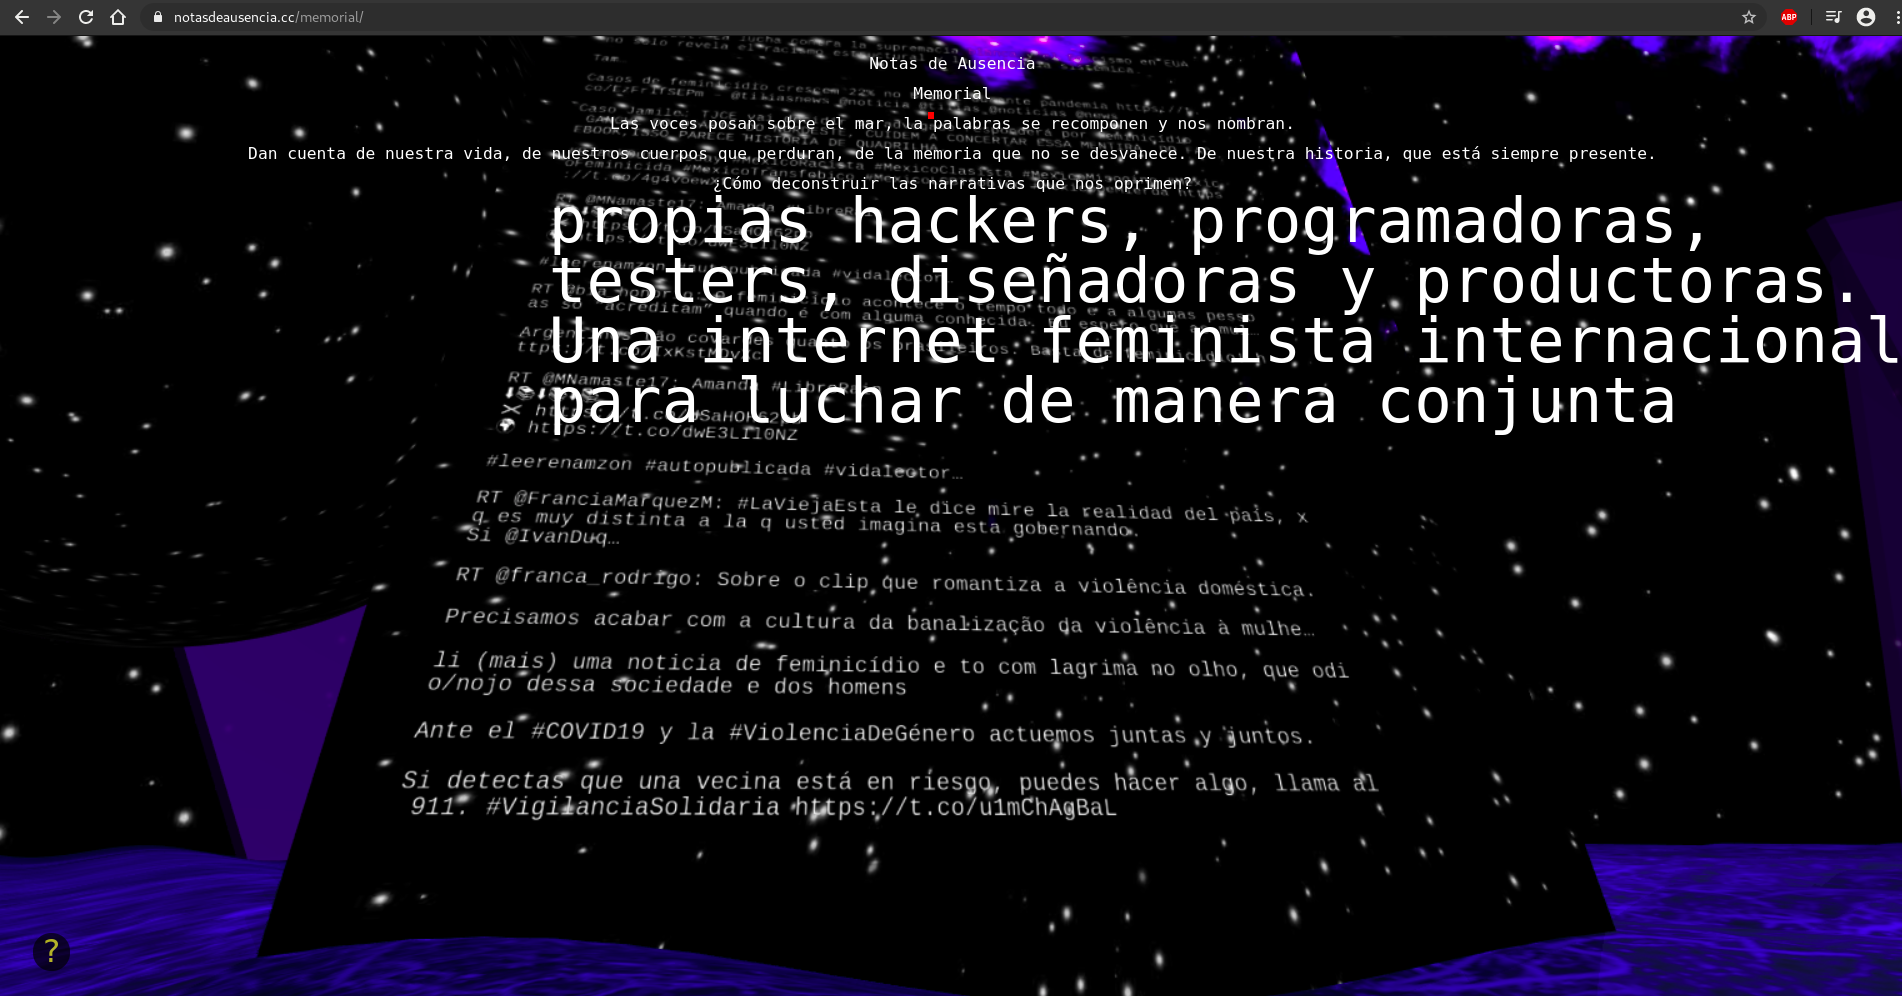
\includegraphics[width=\textwidth]{img/notas02.png}
  \caption{Primera escena. Notas de Ausencia - Marianne Teixido}
  \label{fig:notas1}
\end{figure}

%% Escribir lo que sigue de alguna otra manera. 

\emph{Notas de Ausencia} es un ensayo generativo en la web. Utiliza texto-dato procesado por la computadora como agente resignificante que deconstruye estructuras discursivas para resemantizar la narrativa sobre las desapariciones de mujeres en México y América Latina.

El tiempo y espacio virtual conforman una partitura para la memoria y la denuncia. La narrativa, semi-autónoma, argumenta a partir de textos tomados de tweets, poemarios, libros y artículos feministas que explican desde la teoría las desapariciones forzadas, el feminicidio y la violencia de género. Estos elementos están presentes como texto, imagen y sonido en un espacio tridimensional diseñado a manera de memorial.

\begin{figure}
  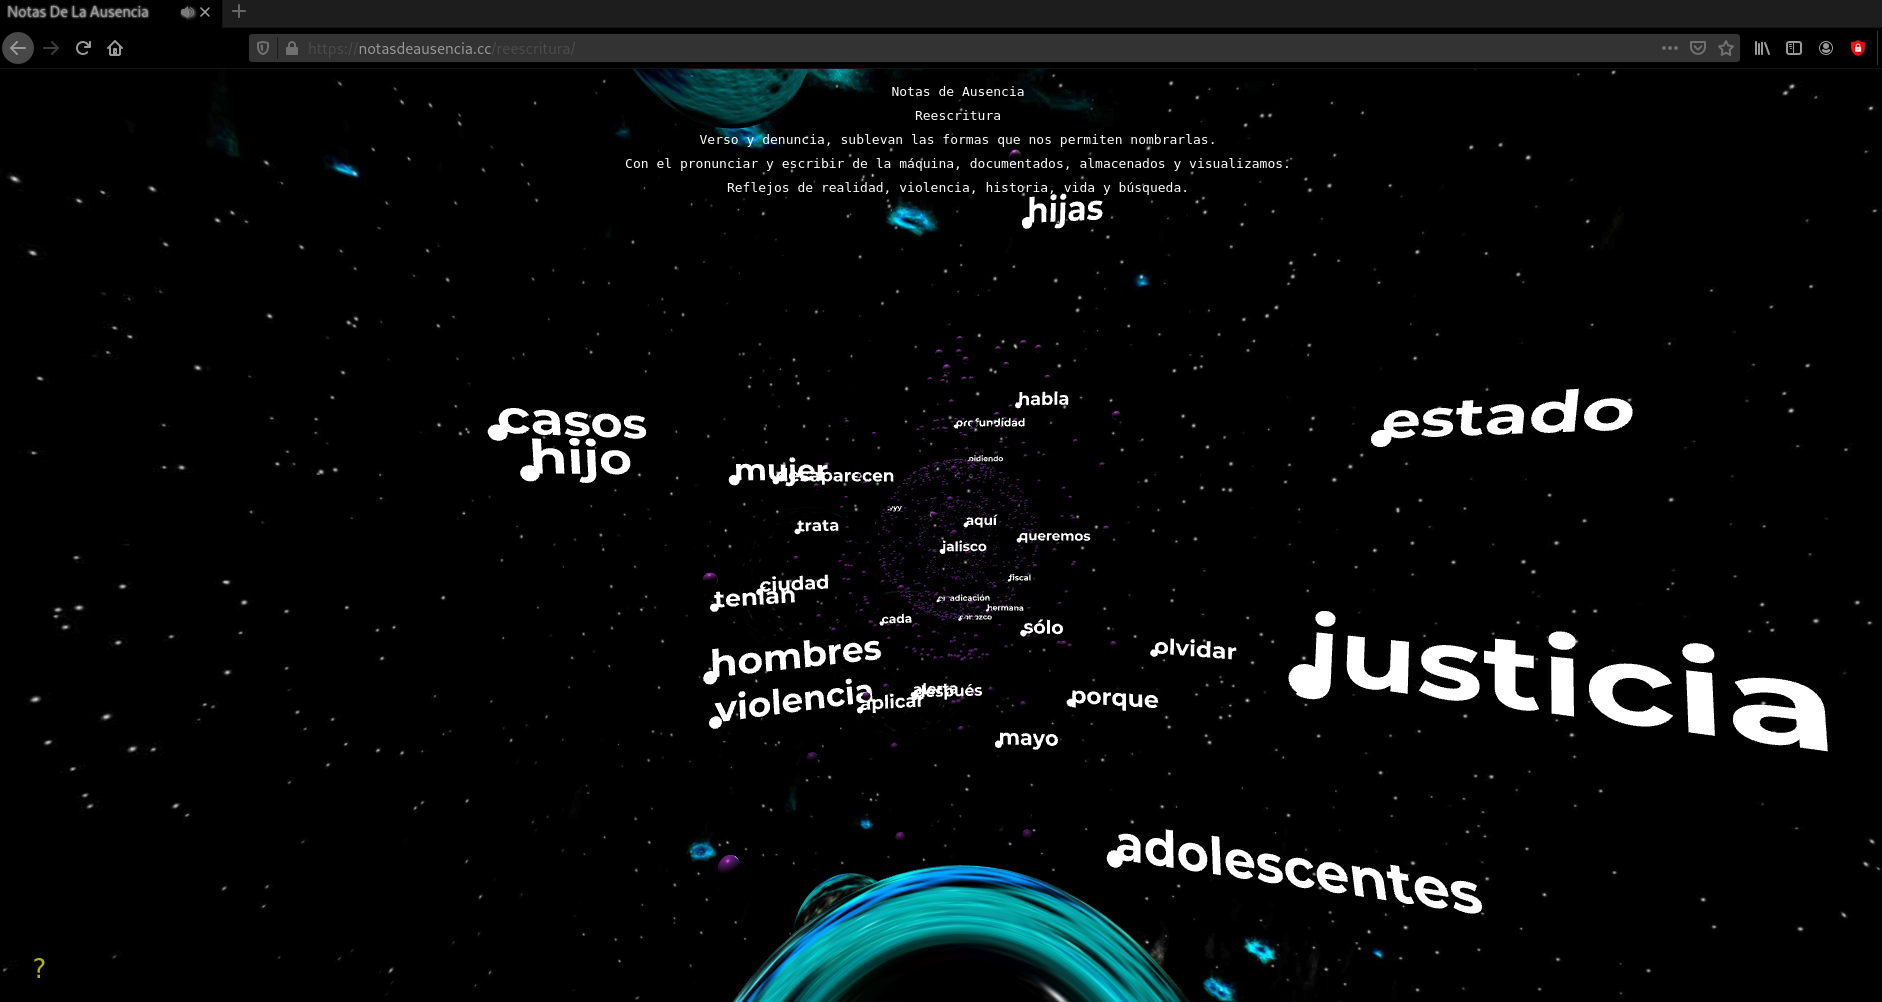
\includegraphics[width=\textwidth]{img/notas03.png}
  \caption{Segunda escena Notas de Ausencia - Marianne Teixido}
\label{fig:notas2}
\end{figure}


La narrativa de la pieza está articulada mediante la intervención de dos bots que interactúan en Twitter. El primero realiza una búsqueda de tuits a partir de un filtro de palabras clave escritas como \emph{hashtags} como: \#MéxicoFeminicida, \#MadresEnBúsqueda, \#ViolenciadeGenero, \#NiUnaMenos, entre otros.\footnote{Actualmente el bot se encuentra activo: \url{https://twitter.com/notasausencia} (Consultado el \today)} Posteriormente, recomparte el tuit que contiene alguno de los \textit{hashtags} de la base de datos previamente delimitada. El segundo bot retoma los textos de los tuits seleccionados y los remezcla para generar un segundo texto automático por medio de cadenas de Markov. 

Esta pieza se realizó en el contexto de la exhibición en línea \textit{Creaciones con Algoritmos: Visualización y Sonificación de Datos} del Centro de Cultura Digital en abril de 2020. Su salida oficial se realizó en video sin embargo, el planeamiento original contempló la creación de un espacio virtual en la web que pudiera visualizar en tiempo real la información viva proveniente de los tweets.

Dos características definieron el diseño de la pieza: ubicación de la pieza en un espacio tridimensional y la interacción y visualización de la información proporcionada por los bots. Para la realización, el proyecto retomó módulos iniciales de \textit{Panorama} y partió del uso de Three.js como un entorno de trabajo que pudiera conectar los dos momentos de la pieza antes descritos. 

A raíz de dicho proceso artístico, el equipo de trabajo generó condiciones técnicas que permitieron la relativa autonomía del servidor requerido para mantener la pieza en línea, que al momento de escritura, permanece activa.

\begin{figure}
  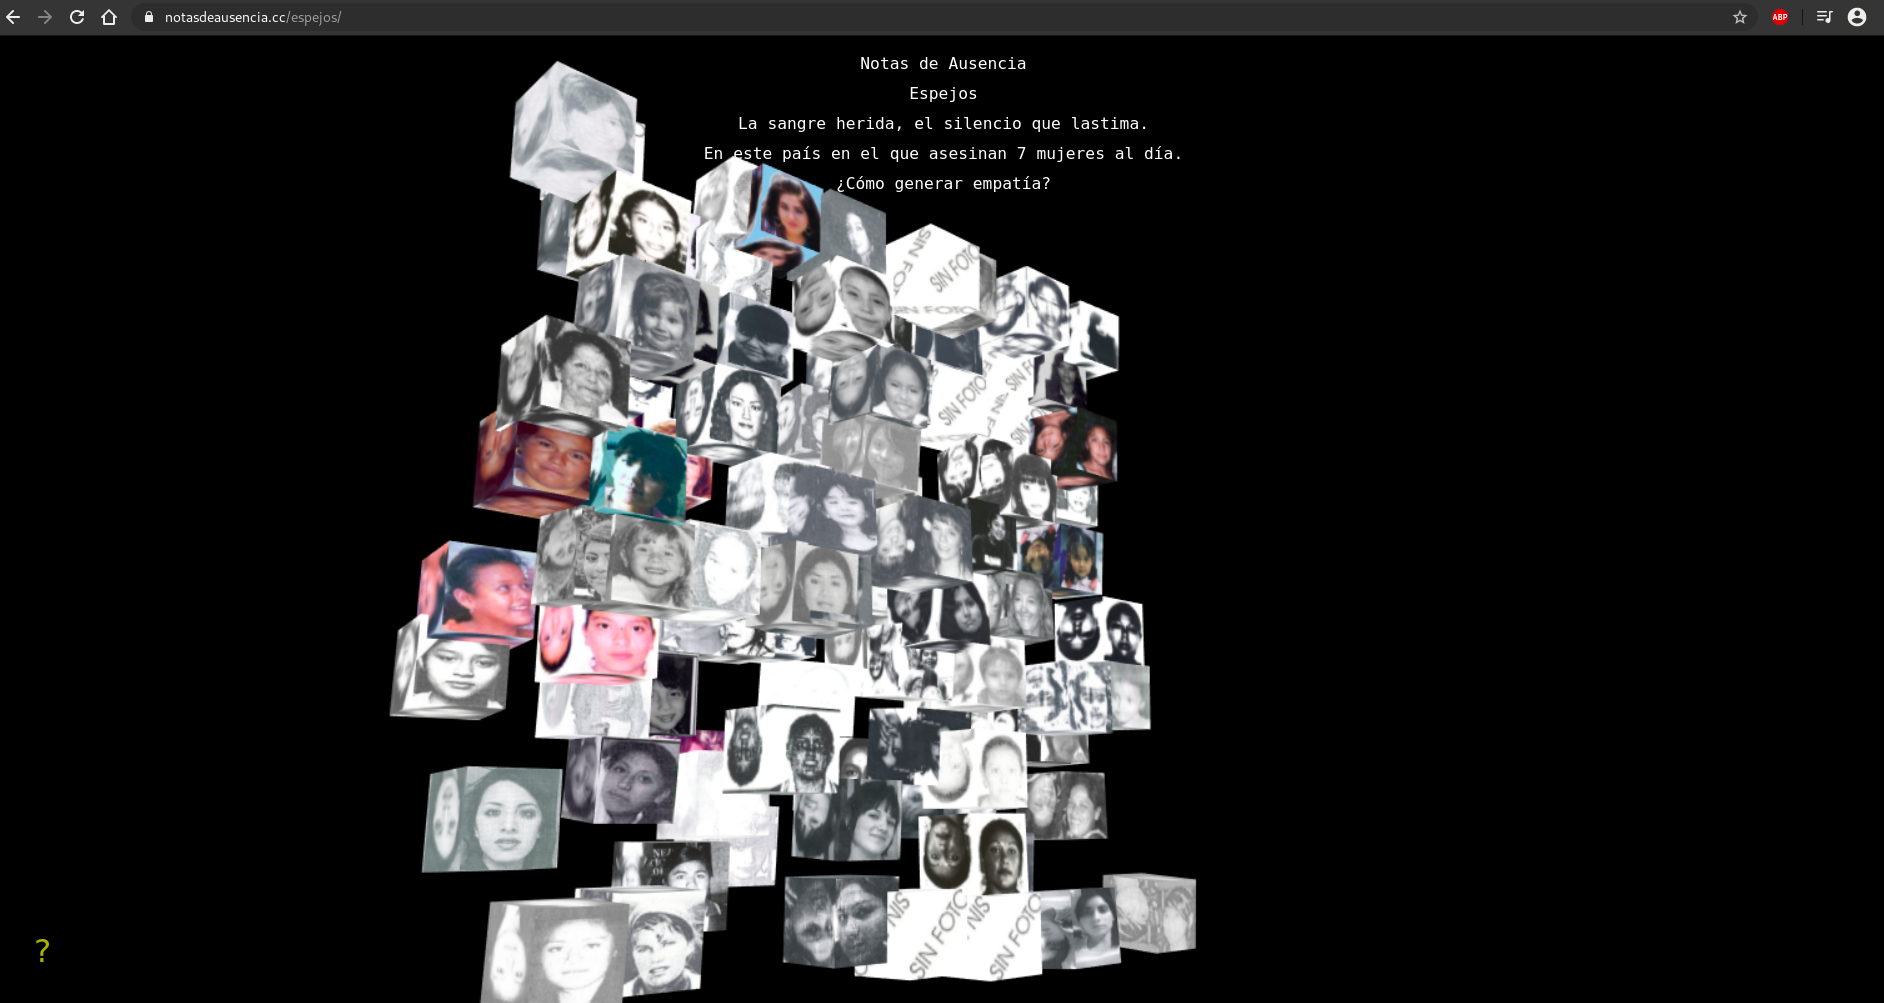
\includegraphics[width=\textwidth]{img/notas04.png}
  \caption{Tercera escena Notas de Ausencia - Marianne Teixido}
  \label{fig:notas3}

\end{figure}

%\begin{figure}[H]
%  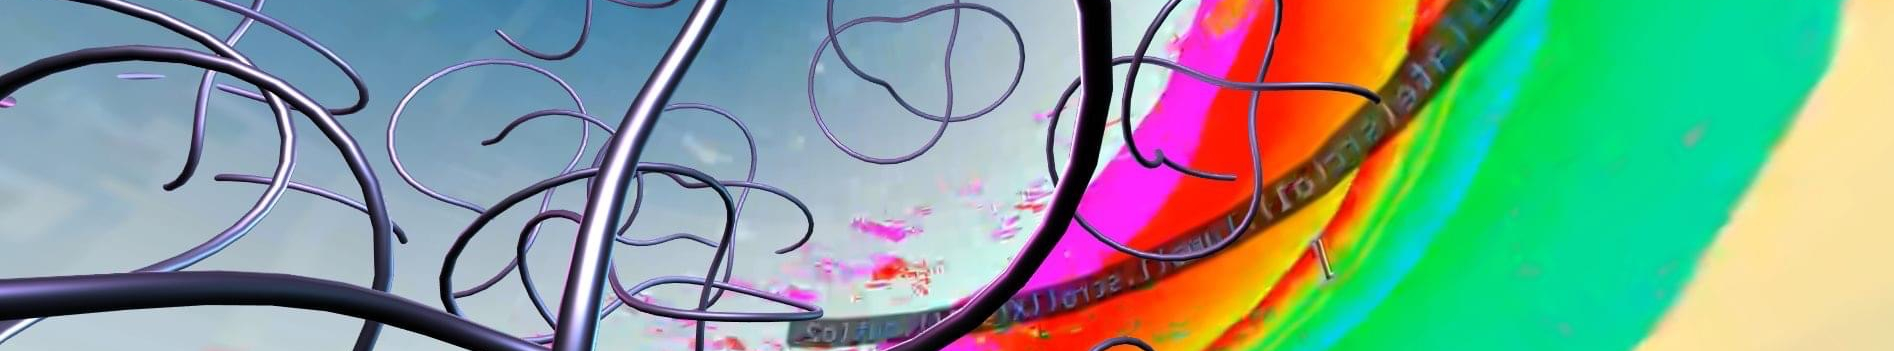
\includegraphics[width=\textwidth]{img/pruebasprofeticas.jpg}
%  \caption{Pruebas proféticas. Visuales: Flor de Fuego}
%\end{figure}

%La transmisión de audio y video fue un aspecto que el planteamiento de \textit{PiranhaLab} buscó solucionar. Es posible utilizar servicios gratuitos o de paga para la transmisión de datos audiovisuales, sin embargo, en menor o mayor medida, el flujo audiovisual generado es analizado y en caso de que se detecte algún extacto de audio proveniente con derechos de autor, el stream es silenciado. Este artículo no busca centrarse en discusiones sobre derechos de autor sino en la usabilidad de un streaming audiovisual. 

 %\color{Fuchsia}

\begin{figure}
  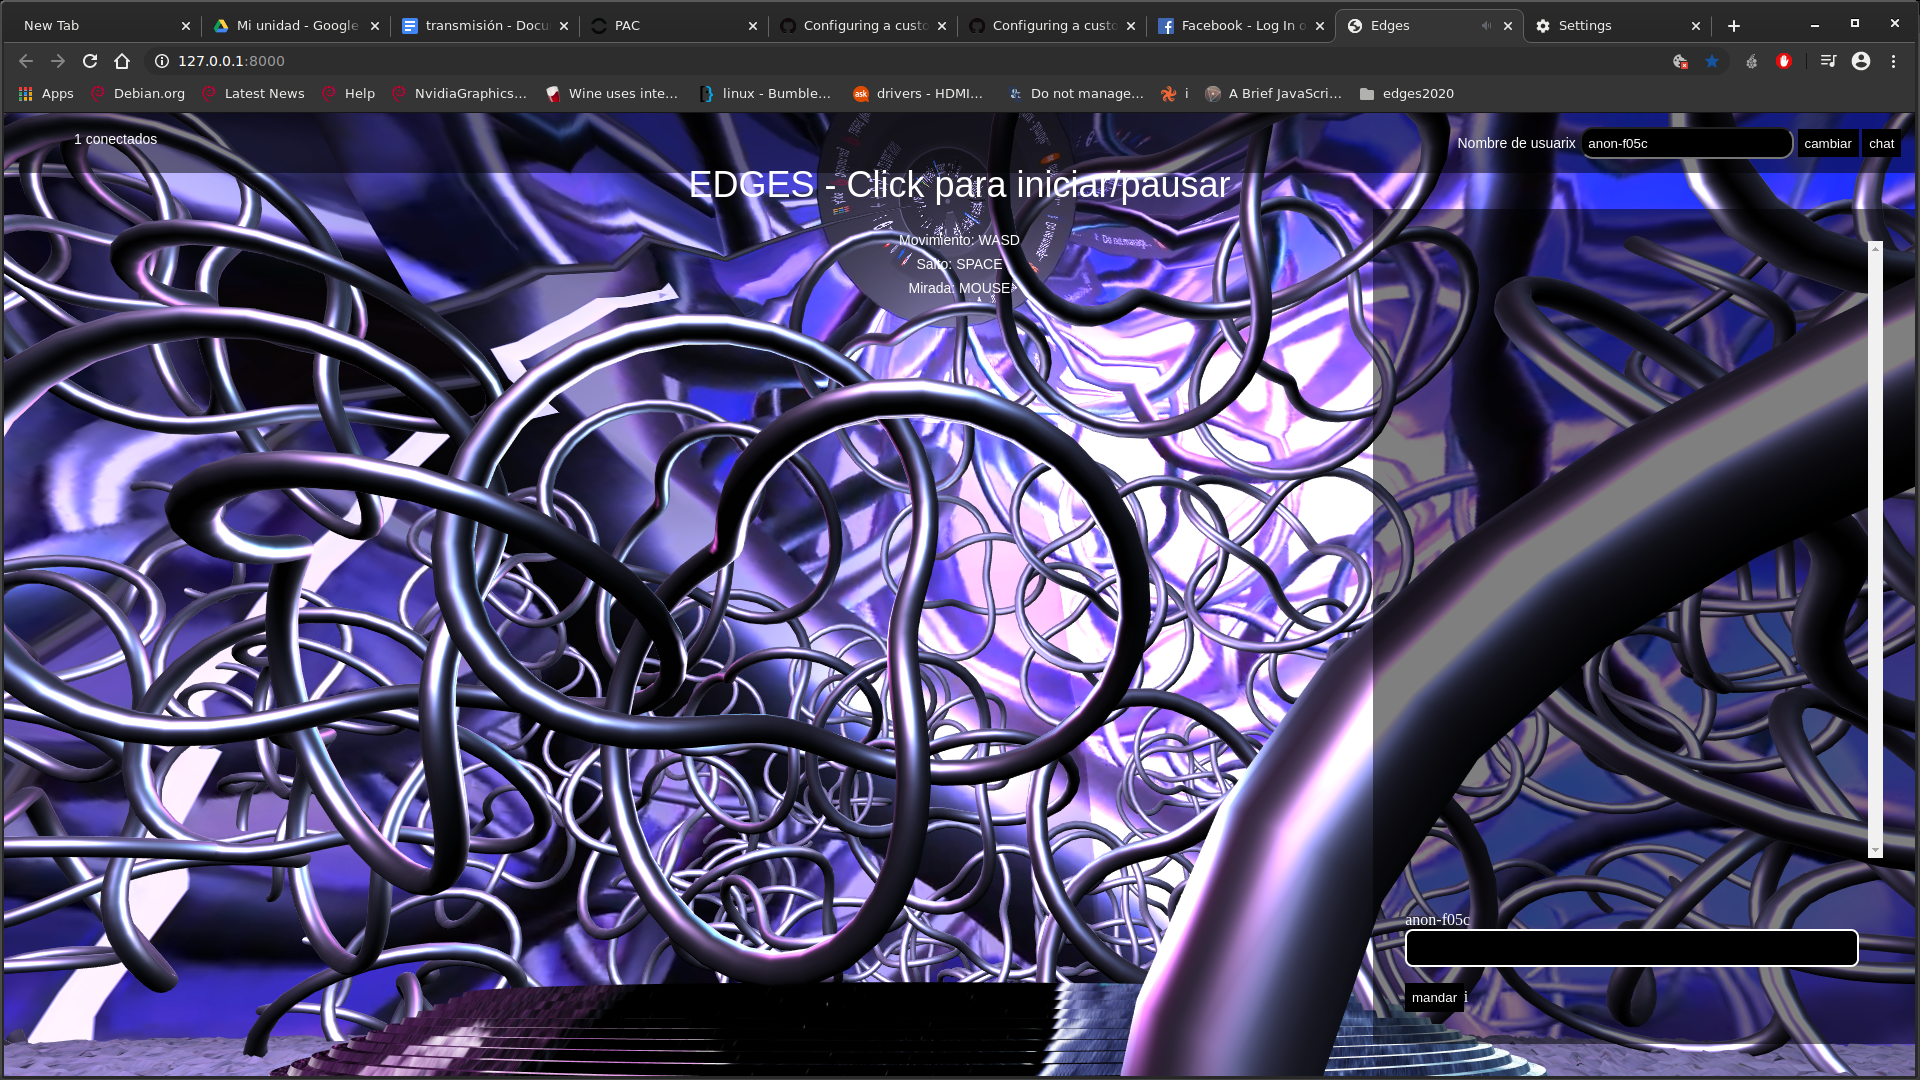
\includegraphics[width=\textwidth]{img/pruebas3.png}
  \caption{Estudio de espacio y retroalimentación para Pruebas Proféticas}
\end{figure}

Como un segundo caso, \textit{Pruebas Proféticas} fue el evento piloto que implementó por primera vez dos tipos de tecnologías específicas: exploración multijugador y \textit{streaming} personalizado. La experiencia con \textit{Pruebas Proféticas} abrió camino para el diseño de la edición 2020 de EDGES. \added[id=EO, comment={Reescritura}]{Este proceso permitió reflexionar en torno a funcionalidad y experimentación como dos posibilidadeas de un continuo para la escritura de software en un marco artístico y performático.} EDGES como plataforma explicita el papel experimental de los actos, la plataforma tecnológica también podría ser experimental e incluso podría desdibujarse en pos de la integración performance-espacio.


\begin{figure}
  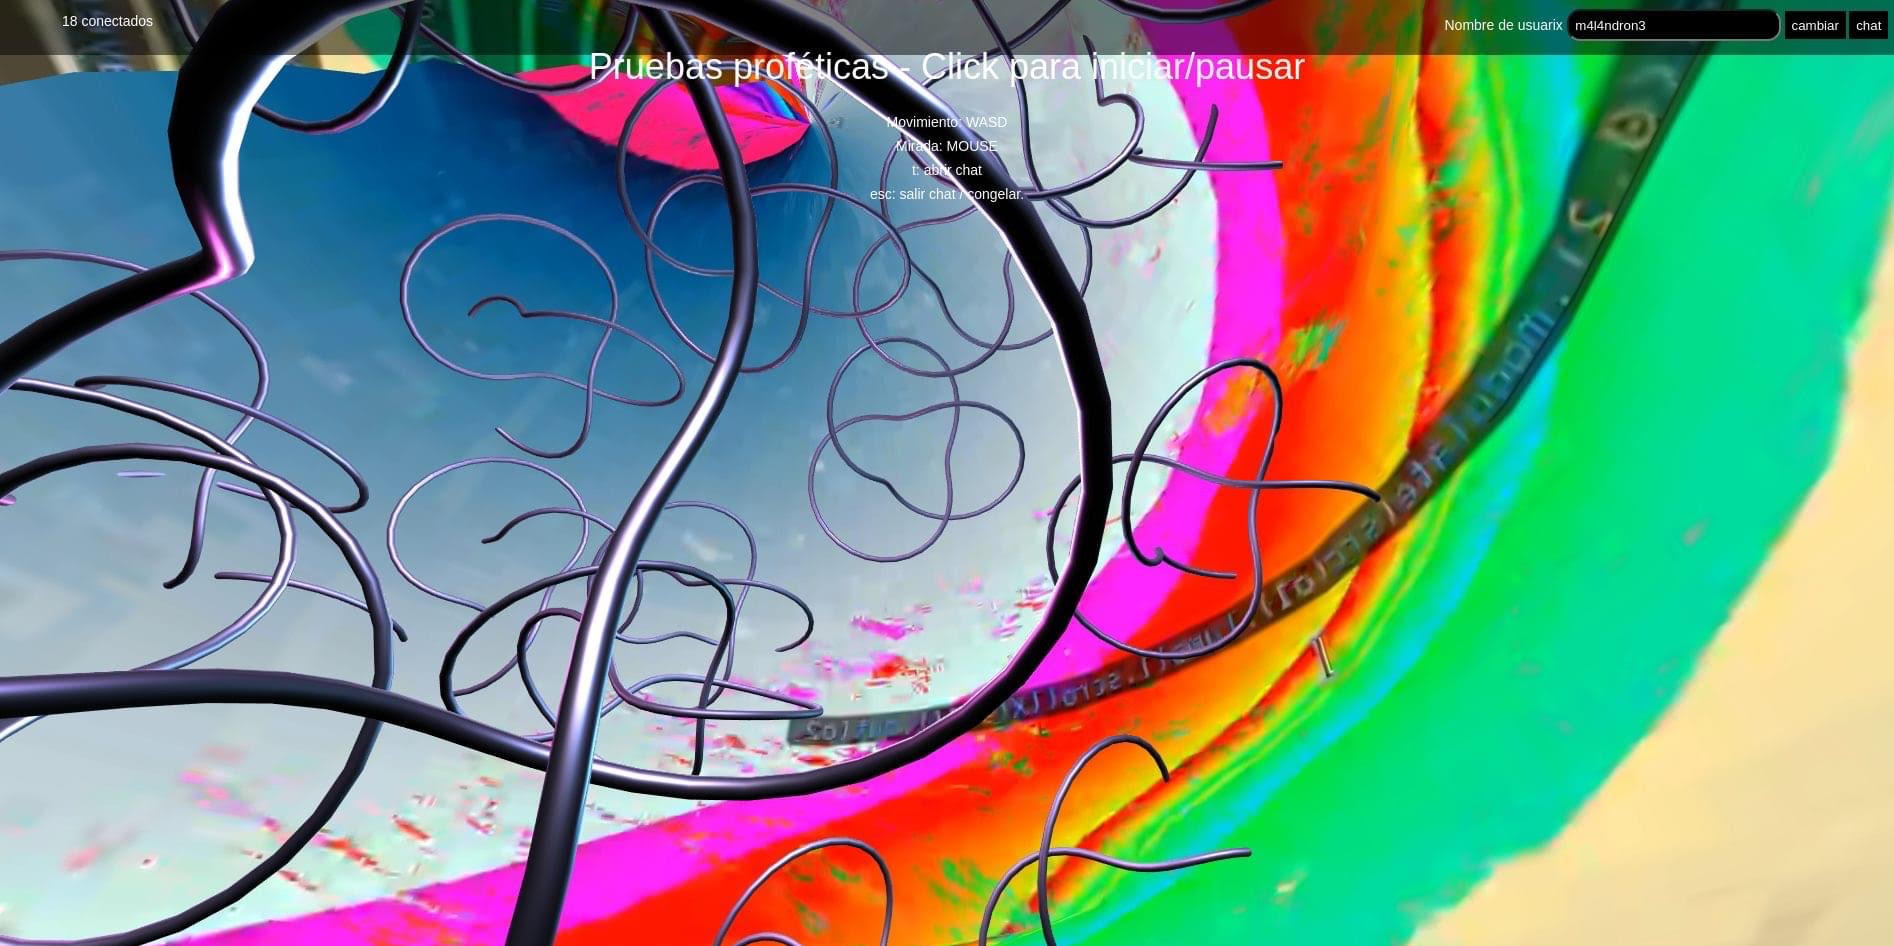
\includegraphics[width=\textwidth]{img/pruebas.jpg}
  \caption{Captura de pantalla de Pruebas Proféticas}
\end{figure}

El concepto curatorial de \textit{EDGES} estuvo definido por Marianne Teixido y guardó una estrecha relación con los planteamientos de \textit{Notas de Ausencia}. Considera las posibilidades de creación planteadas desde el feminismo interseccional, perspectiva desde la cual se problematiza el uso de la tecnología teniendo en consideración las condiciones de raza, género y clase. También es posible articular práctica y curaduría con una crítica a las herramientas hegemónicas previamente dadas para apuntar a la creación de herramientas personalizadas y críticas, construidas desde dinámicas de organización colectiva y conocimientos situados. \textit{EDGES 2020} como propuesta curatorial contempla la participación en su mayoría de mujeres y personas no binaries. Las obras dialogan con las hibridaciones e-corporales en espacios virtuales ficcionados desde las subjetividades feministas y transfeministas que toman internet como territorio y espacio de intercambio cultural.

\iffalse
- Uso de espacios tridimensionales 
- Bots y literatura 
- Datos que transforman el espacio   
- Ensayos digitales en la web
- cyberfeminisimo
- audio virtualmente posicionado 
- streaming de audio y video sin plataformas privativas - decisiones de optimización
- Según yo aquí usamos icecast y liquid soap 
- Inicios de multiplayer
\fi

\begin{figure}
  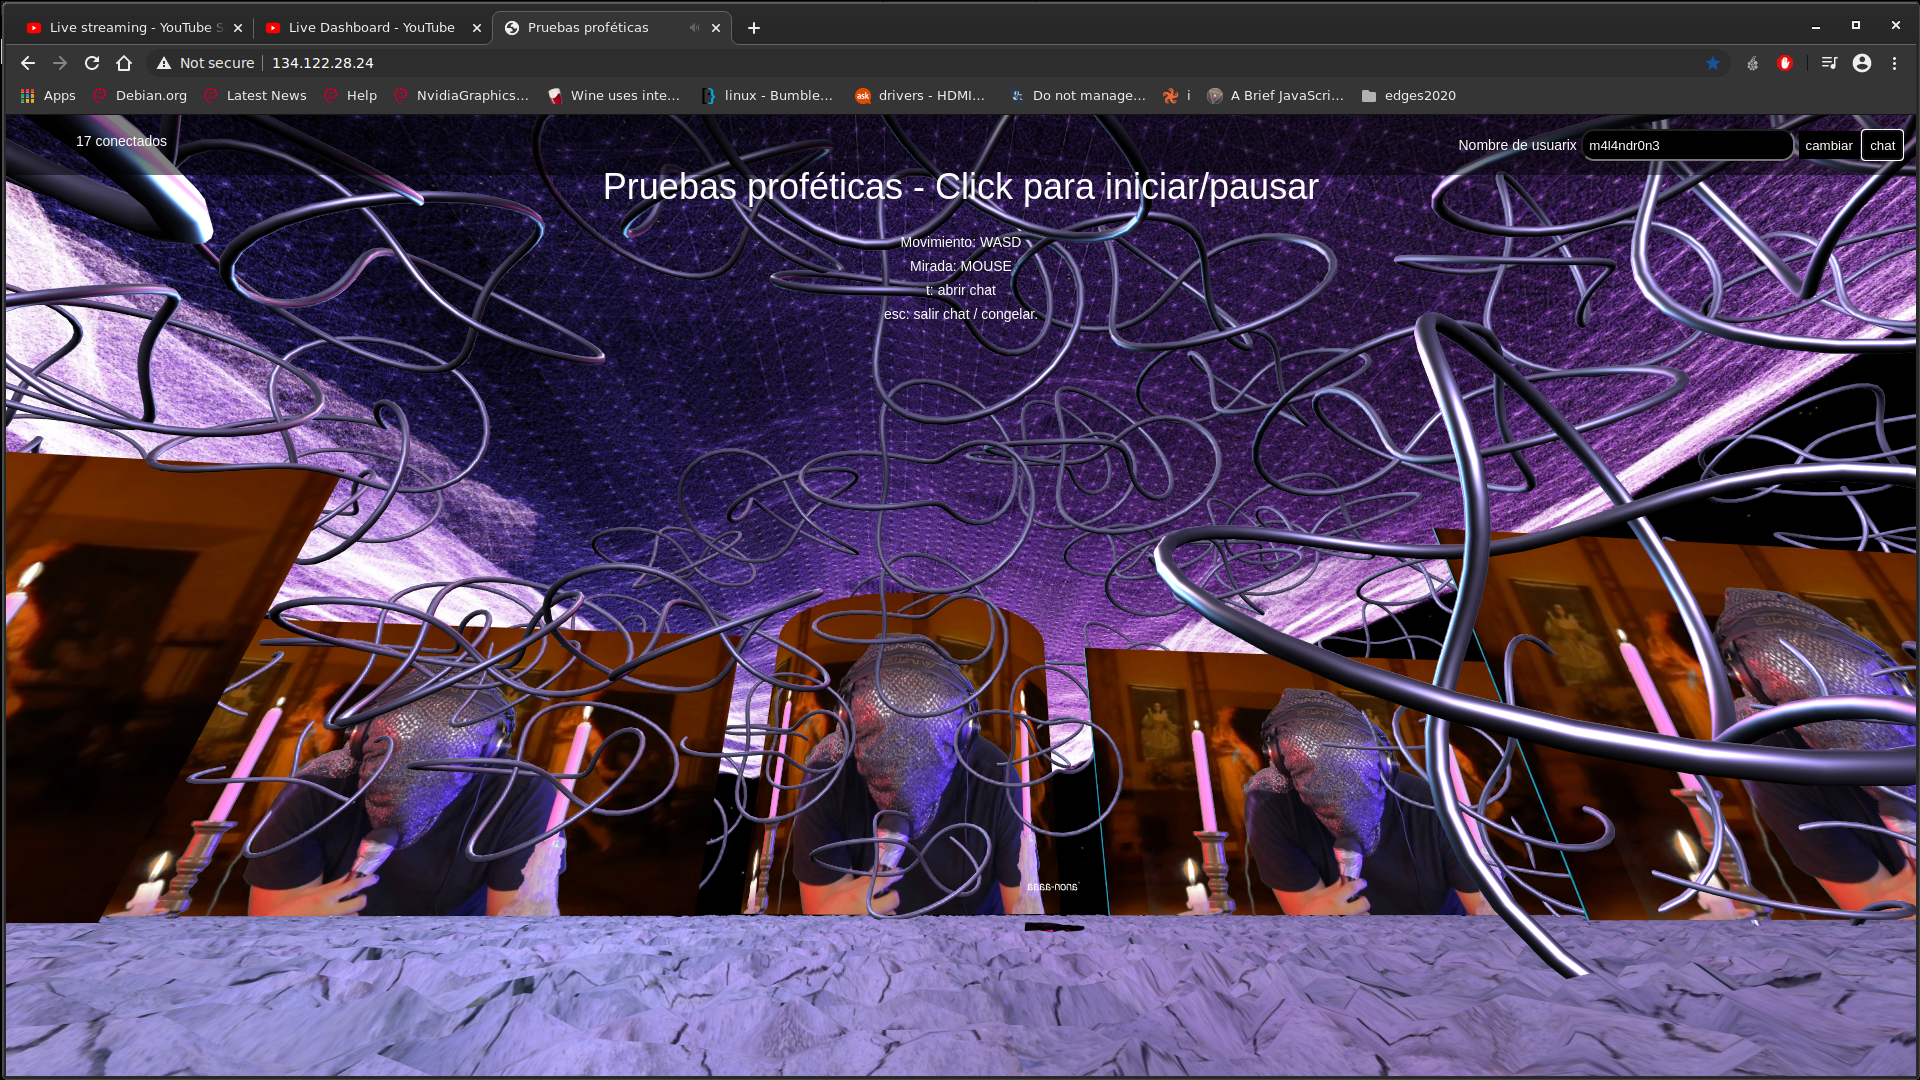
\includegraphics[width=\textwidth]{img/pruebas2.png}
  \caption{Captura de pantalla de Pruebas Proféticas}
\end{figure}
% \color{black}
 % Primera parte que describe resultados. Casos elegidos: Notas de Ausencia y Pruebas proféticas

\section*{Contemplación y EDGES} % Espacio para hablar del proyecto de (acomplete) de Dorian

\begin{itemize}
\item Distopía
\item domo 
\item Underborders
\item Milena y Concepción
\item setInterval()
\item Contemplación del fin del Mundo
\item sistemas mixtos
\item espacio y performance fusionados en Contemplación
\end{itemize}


La contemplación del fin del mundo es un performance a modo de ejuego por ser el último evento de la serie de conciertos edges, dando por finalizado de manera simbólica, destruyendo el escenario.
Los asistentes podían presenciar el fin del mundo a modo de destrucción del escenario, inundaciones, objetos celestiales y finalmente la dispersión de los colores del escenario, dejando los objetos sin razgos reconocibles.

La idea principal sirvió como vehículo para la exploración del espacio como característica del performance, el mundo explorable, la persecución en forma de figuras celestiales que ocupaban todo el espacio o que se expandían e iluminaban todo así como las inundaciociones, además del uso de pantallas distribuidas a lo largo de todo el mundo, permitiendo a los usuarios presenciar el performance desde cualquier ubicación.

Se puede destacar de este concierto, el uso de acciones colectivas lanzadas por el artista, quien durante el trascurso del evento podía cambiar las características del ambiente de manera similar entre los participantes, teniendo todos una experiencia compartida homogénea y en el momento, además del uso de framework externos  para la creación de visuales.
Las dificultades de las experiencias compartidas radican en la sincronización de eventos, tanto para los usuarios que ingresan desde el inicio o los usuarios ocasionales, sin importar ubicación geográfica o dispositivo.
Esta posibilidad agrega la capacidad de interacción de parte del artista, generando situaciones que añadan dinámica al juego, donde los asistentes podrían participar más allá de ser meros observadores
  % Segunda parte que describe resultados. Casos elegidos: EDGES y La contemplación del Fin del Mundo
% 
 % Tercera parte que describe resultados. Casos elegidos: threecln (en proceso) y 4nt1 (en proceso)
% 
\section*{Discusión}

Los eventos realizados en esta diversidad de plataformas han utilizado ligas a internet que de acuerdo a la fecha consultada, redireccionan a distintos espacios virtuales. A diferencia de los sitios que utilizan texto y entornos de programación web como HTML, la mezcla de módulos y el uso de frameworks dedicados que utilizan renderizadores 3d como webGL, motores de audio como Web Audio API o plataformas de transmisión de audio y video personalizadas y efímeras dificultan la documentación convencional. La labor se complica cuando el mantenimiento de estos espacios sobrepasa los ealcances temporales o económicos del proyecto. El reto metodológico que esto supone es un asunto pendiente para las investigaciones que hacen referencia a tecnología. En este sentido, la referencia a repositorios de código públicos podrían arrojar soluciones para la documentación y arqueología de los desarrollos tecnológicos. Una alternativa para la documentación de estos procesos es Wayback Machine.  % Indagar sobre esto

% Referencias a la consecuencia y no al objeto por sí mismo 

La discusión en torno a la escritura de software inicia con la perspectiva prostética y termina problematizando las ideas que orbitan en torno a la cajanegrización de cara a la idea del trabajo socialmente invertido en esta actividad.

Manifiestos, posturas políticas y alternativas en la organización que dialogan con la escritura de software como desarrollo tecnológico y como acto creativo. Por ejemplo \textit{live coding} y la transparencia de los procesos o el uso de interfaces de texto \citep{collinsLivecoding}, el manifiesto de una servidora feminista \citep{feministserver} o la arquitectura de intercambio de información basada en pares (p2p) que persigue la distribución y la descentralización y que incluso puede extenderse al autocuidado y formas alternativas de expresar relaciones sociales en red. 

Estas perspectivas pueden incluso extenderse hacia una postura para la investigación de tecnología y el papel que juegan en la política de los espacios físicos y virtuales, como el cuarto propio \citep{cuartopropio} o el buen conocer (cita platohedro).  

Funcionalidad y experimentación como dos posibilidades de un continuo para el la escritura de software en un marco artístico y performático. EDGES como plataforma explicita el papel experimental de los actos, la plataforma tecnológica también podría ser experimental e incluso podría desdibujarse en pos de la integración performance-espacio bajo la misma premisa de la experimentación. 

La gamificación (gamification) tácita en la escritura de proyectos como \textit{Panorama}. Esto implica 1) tecnología, por ejemplo pantallas, combinaciones de teclas para la exploración de espacios pero también dispositivos de realidad virtual, 2) diseño visual y sonoro de los espacios, objetos digitales en espacios tridimensionales, audio inmersivo, 3) intercambio de información para la co-presencia en tiempo real dentro de espacios digitales o el multijugador e incluso 4) narrativas e imaginarios a explorar. 
 
\iffalse

- manifiestos y posturas políticas > live coding y servidora feminista 
- Diferencias con respecto a otros espacios
- Discusión sobre lo digital, los nuevos medios y la virtualidad. 
- Giro de los nuevos medios
- Agotamiento del formato
- funcionalidad - experimentación 
- Arqueología en internet (cosas que ya tienen tiempo y cosas recientes). 
- El papel de los videojuegos gamización
- Lo barroco y el artículo de electroacústica. 

\fi
 % Como los resultados se vinculan con las reflexiones y perspectivas externas al artículo.

\section*{Conclusiones}

% Este espacio podría estar bueno para enunciar posibles vetas de investigación a partir de lo que paso. Podriamos aclarar que fue un proyecto práctico que detonó reflexiones e ideas que se pueden desarrollar más adelante. Aquí también puede anunciarse el trabajo con three y anti 

% La pregunta principial sería: ¿Se cumplió la hipótesis/premisa del software escrito? 

% Comenté lo de abajo, creo que es redundante

% Los usuarios pudieron compartir una experiencia ligera para el navegador de manera co-presencial, aprovechando las posibilidades de las tecnologías de transmisión de audio y video. Destacamos la importancia de plantear soluciones compartibles en lo que respecta a la transmisión de audio-imagen. La escritura de esta parte de \textit{Panorama} fue utilizado en el marco de otros eventos y ciclos.

%El proyecto no tuvo un plan de acción específico para la realización de mediciones durante los conciertos, a pesar de que el control del servidor lo permitió. Sin embargo, la lectura de información a partir de una simulación del evento arroja datos importantes en este sentido.

%Sobre las impresiones del público, fue posible realizar un cuestionario durante \textit{Pruebas Proféticas}. 

%La importancia de una infraestructura tecnológica y social. Esto se puede entretejer a partir de decisiones curatoriales que vinculan potencial tecnológico con alianzas entre actores. 

%Del lado teórico es necesario convenir y reforzar un corpus de conceptos para la investigación sobre Tecnología Musical. Detección de campos y persectivas de investigación: las agencias que están presentes en eventos que se desenvuelven con tecnología.


%Las consecuencias estéticas, tecnológicas e investigativas de estos eventos apuntan a la necesidad de establecer un corpus de conceptos y perspectivas que posibiliten la observación de nuevas prácticas artísticas con medios \citep{shankenCanon} que implican la interpretación musical digital y que se desborda a otros campos. Esta intención podría incluir la estética de estas prácticas, la programación del software que las posibilita, su condición como software escrito y ejecutado \citep{speakingCode} y las consecuencias sociales y políticas de la distribución en red. % Esto podría estar después 

%Los eventos realizados en la diversidad de plataformas anteriormente descrita han utilizado ligas a internet que de acuerdo a la fecha consultada, redireccionan a distintos espacios virtuales. A diferencia de los sitios que utilizan texto y entornos de programación web como HTML, la mezcla de módulos y el uso de frameworks dedicados que utilizan renderizadores 3d como webGL, motores de audio como Web Audio API o plataformas de transmisión de audio y video personalizadas y efímeras dificultan la documentación convencional. La labor se complica cuando el mantenimiento de estos espacios sobrepasa los alcances temporales o económicos del proyecto. El reto metodológico que esto supone es un asunto pendiente para las investigaciones que hacen referencia a programas de computadora como recurso. En este sentido, la referencia a repositorios de código públicos podrían arrojar soluciones para la documentación y arqueología de los desarrollos tecnológicos. Una alternativa posible es \textit{Wayback Machine}\footnote{``\textit{The Wayback Machine} es una iniciativa de Internet Archive para construir una librería digital de sitios de Internet y otros artefactos culturales en formato digital''. \url{http://web.archive.org/} (Consultado el \today)} y en general, reestructurar la forma en la que se documenta y experimentan los sitios web. 

%Estas perspectivas pueden extenderse hacia una postura para la investigación de tecnología y el papel que juegan en la política de los espacios físicos y virtuales, como el cuarto propio \citep{cuartopropio} o el buen conocer \citep{plato}. Podríamos relacionar estos procesos con el giro de los nuevos medios descrito por \cite{manovichlanguage}, las implicaciones sociales de este giro y sobre todo, las consecuencias estéticas que a partir de este se abren y desenvuelven en el performance musical por medio de la computadora y otras prácticas afines. 

%Destacamos el giro de los nuevos medios como un cambio de paradigma que la tecnología musical debe considerar por las implicaciones de los usos/críticas de las tecnologías de la información, las tendencias para la resolución de problemas relacionados con gestión de datos y las consecuencias estéticas que a veces se empalman y otras rebasan a la música y las perspectivas de investigación asociadas a esta disciplina. El rodeo o la realización de un motivo tecnológico como una perspectiva de investigación que pueda aportar en el aspecto tecnológico y teórico-metodológico, sobre todo en campos que lo permiten como humanidades, artes y específicamente, investigación que implica música y expresiones audiovisuales con tecnología.

%\color{Fuchsia}

%A manera de cierre, consideramos que la observación y la investigación podría extenderse a manifiestos, posturas políticas y alternativas en la organización que dialogan con la escritura de software como desarrollo tecnológico y como acto creativo. Tal es el caso de la práctica de \textit{live coding} y la transparencia de los procesos o el uso de interfaces de texto \citep{collinsLivecoding}, el manifiesto de una servidora feminista \citep{feministserver} o la arquitectura de distribución de información par a par\footnote{\textit{P2P} (par a par) por sus siglas en inglés.  ``La arquitectura de una red distribuida puede ser llamada Par a Par (P-to-P, P2P, ...)   si los participantes comparten una parte de los recursos de su propio software (poder de procesamiento, capacidad de almacenamiento, capacidad de conexión a la red, impresoras,...) Estos recursos compartidos son necesarios para proveer el Servicio y el contenido ofrecido por la red... Estos son accedidos por otros pares directamente sin pasar por entidades intermediarias." \citep{p2p}} que persigue la distribución y la descentralización en redes que posibilitan espacios virtuales \citep{cyberspace} y que incluso puede extenderse al autocuidado y formas alternativas de expresar relaciones sociales en red \citep{dwc} o desmantelar y reconfigurar tecnologías en relación a la estética, a la tecnología y a la organización social distribuida. 


El navegador, como una tecnología accesible en términos de recursos de la computadora y de dispositivos o instalaciones adicionales, permitió la escritura de espacios inmersivos con \textit{Panorama}. Consideramos que la optimización de estos espacios para dispositivos móviles y la exploración extendida para la transmisión de datos bajo la lógica de la compartición par a par\footnote{\textit{P2P} (par a par) por sus siglas en inglés.  ``La arquitectura de una red distribuida puede ser llamada Par a Par (P-to-P, P2P, ...)  si los participantes comparten una parte de los recursos de su propio software (poder de procesamiento, capacidad de almacenamiento, capacidad de conexión a la red, impresoras,...) Estos recursos compartidos son necesarios para proveer el Servicio y el contenido ofrecido por la red... Estos son accedidos por otros pares directamente sin pasar por entidades intermediarias." \citep{p2p}} son puntos que quedan pendientes para la escritura e investigación futuras. 

A diferencia de los sitios que utilizan texto y entornos de programación web como HTML, la mezcla de módulos y el uso de frameworks dedicados que utilizan renderizadores 3d como webGL, motores de audio como Web Audio API o plataformas de transmisión de audio y video personalizadas y efímeras dificultan la documentación convencional. La labor se complica cuando el mantenimiento de estos espacios sobrepasa los alcances temporales o económicos del proyecto. El reto metodológico que esto supone es un asunto pendiente para las investigaciones que hacen referencia a programas de computadora como recurso de investigación. En este sentido, la referencia a repositorios de código públicos podrían arrojar soluciones para la documentación y arqueología de los desarrollos tecnológicos. Una alternativa posible es \textit{Wayback Machine}\footnote{``\textit{The Wayback Machine} es una iniciativa de Internet Archive para construir una librería digital de sitios de Internet y otros artefactos culturales en formato digital''. \url{http://web.archive.org/} (Consultado el \today)} y en general, reestructurar la forma en la que se documenta y experimenta la web. 


El trayecto de investigación involucrado en \textit{Panorama} arrojó motivaciones para la realización de piezas que se ejecuten entre espacio, tiempo e interpretación. Al momento de escritura hay dos proyectos que atienden estos aspectos y que pueden extender la discusión: THREE.studies\footnote{Versión fija en la web y repositorio: \url{http://threecln.piranhalab.cc/} \url{https://github.com/EmilioOcelotl/THREE.studies}} y 4NT1.\footnote{Versión web en construcción. Repositorio: \url{https://github.com/EmilioOcelotl/anti}} Teniendo en cuenta la extensión de la realización estética y tecnológica, una posible agenda de creación investigación podría tener en cuenta la colaboración y la realizacion de piezas en un contexto post-pandemia que podría acoplar aspectos de la co-presencia física y de la interacción digital. 


El proceso de escritura e investigación presente en \textit{Panorama} permitió enlazar la documentación, propia y externa, con la perspectiva de investigación. Consideramos que la investigación artística y la metáfora como estrategias posibles para conceptos que atraviesan lo estético, lo tecnológico y lo investigativo. Proyectos de investigación, creación y escritura de software futuros podrían tener en cuenta el uso de conceptos transversales. 

Estas perspectivas pueden extenderse hacia una postura para la investigación de tecnología y el papel que juegan en la política de los espacios físicos y virtuales, como el cuarto propio \citep{cuartopropio} o el buen conocer \citep{plato}. Podríamos relacionar estos procesos con el giro de los nuevos medios descrito por \cite{manovichlanguage}, las implicaciones sociales de este giro y sobre todo, las consecuencias estéticas que a partir de este se abren y desenvuelven en el performance musical por medio de la computadora y otras prácticas afines. 

Destacamos el giro de los nuevos medios como un cambio de paradigma que la tecnología musical debe considerar por las implicaciones de los usos/críticas de las tecnologías de la información, las tendencias para la resolución de problemas relacionados con gestión de datos y las consecuencias estéticas que a veces se empalman y otras rebasan a la música y las perspectivas de investigación asociadas a esta disciplina. El rodeo o la realización de un motivo tecnológico como una perspectiva de investigación que pueda aportar en el aspecto tecnológico y teórico-metodológicoa la investigación que implica música y expresiones audiovisuales con tecnología.

%\color{Fuchsia}

A manera de cierre, consideramos que la observación podría enlazarse con manifiestos, posturas políticas y alternativas en la organización que dialogan con la escritura de software como desarrollo tecnológico y como acto creativo. Tal es el caso de la práctica de \textit{live coding} y la transparencia de los procesos o el uso de interfaces de texto \citep{collinsLivecoding}, el manifiesto de una servidora feminista \citep{feministserver} o la arquitectura de distribución de información par a par, que persigue la distribución y la descentralización en redes que posibilitan espacios virtuales \citep{cyberspace} y que incluso puede extenderse al autocuidado y formas alternativas de expresar relaciones sociales en red \citep{dwc} o desmantelar y reconfigurar tecnologías en relación a la estética, a la tecnología y a la organización social distribuida. 



% Objetivo de la investigación: realización de sistemas ligeros que puedan ser accesibles con uan tecnología relativamente económica para la computadora para el navegador. Los eventos pudieron realizarse, sin dificultades, quedo pendiente la resolución de una versión para el navegador. 

% Objetivo secundario: documentación de software y del proceso 

% Agenda de enunaciación de trabajos y reflexiones para el futuro.

% Antes que nada, la perspectiva de observación / investigación. ¿Por qué esto tendría que estar al inicio? Diferencia entre documentación y observación 

% Documentación propia y ajena. 

% Software escrito en el contexto de trabajos y piezas post pandemia

% Aquí puede ir lo de THREE.studies y Anti 

% Reflexiones pendientes que pueden extenderse en otros momentos de investigación 

% Consecuencias no buscadas que se empalman con el proyecto. Idea interesante proveniente de Bruno Latour: es tiempo de girar de un paradigma que abierta o tácitamente refiere a la escala de recursos de la computadora. Si podemos trasladar esta lógica a una economía de los recursos de la computadora, no es tiempo ya de dar un giro que deje de hacer patente lo económico para dar paso a lo ecológico. 

%%%%%%%%%%%%%%%%% Pendiente: servidores, autogestión y cuerpós 

% Hacerse cargo de la gestión de los datos y de los servidores tiene que ver con los cuerpos, El cuerpo es infraestructura que posibilita el funcionamiento de los servidores.

% Servidores de todas formas generan consecuencias ecológicas > cambios significativos tendrían que ser de empresas y no tanto proyectos chiquitos. 

% Reducción de energía > responsabilidad de datos

% Cuerpo medio e interfaz como se articulan > Hans Belting > Imagen medium y cuerpo. Un nuevo acercamiento a la iconología > ¿Imágenes tradicionales? 

% PeerTube transitar del modo servidor a la forma de estructurar la experiencia en modo p2p
 % ¿Se cumplió la premisa/hipótesis descrita en Diseño y Escritura? ¿Qué otras cosas surgieron?

\theendnotes % El artículo usa notas al final del texto. Aquí aparecen hipervínculos y conceptos de apoyo. Conceptos 

%\nocite{interactiveDigitalMusic}
% \nocite{speakingCode} 

\addcontentsline{toc}{chapter}{\protect\numberline{}Referencias}%
\bibliography{bib/panBib}{} % Referencias bibliográficas y repositorios en Git como referencias en la web.
\bibliographystyle{apalike-es}

\end{document}
